\documentclass[border=2pt]{standalone}
% Shared TikZ style contract for every schematic figure in this paper.
% Each schematic is a standalone document that \input's this file, so the
% schematics and the matplotlib data figures form one visual system.
%
% Colours are the same Okabe-Ito values as figures/scifig_style.py.

% No font package: the manuscript class sets the body in Computer Modern, so
% the schematics inherit the same family by loading nothing here.
\usepackage{amsmath,amssymb}
\usepackage{tikz}
\usetikzlibrary{arrows.meta,positioning,calc,fit,backgrounds,shapes.geometric,
                shapes.multipart,patterns,decorations.pathreplacing,matrix}

% ---------- Notation shared with the manuscript ----------
% Kept in sync with the definitions in main.tex so that a symbol means the
% same thing in a schematic as it does in the body.
\newcommand{\Cmax}{C_{\max}}
\newcommand{\Zcost}{Z}
\newcommand{\Nb}{\mathcal{N}}

% ---------- Okabe-Ito colour-blind-safe palette ----------
\definecolor{oiblue}{RGB}{0,114,178}
\definecolor{oiorange}{RGB}{230,159,0}
\definecolor{oigreen}{RGB}{0,158,115}
\definecolor{oivermilion}{RGB}{213,94,0}
\definecolor{oipurple}{RGB}{204,121,167}
\definecolor{oisky}{RGB}{86,180,233}
\definecolor{oiyellow}{RGB}{240,228,66}
\definecolor{oigray}{RGB}{110,110,110}

% ---------- Shared node and arrow styles ----------
\tikzset{
  block/.style={draw, rounded corners=2pt, minimum height=6.5mm, minimum width=17mm,
                align=center, font=\footnotesize, fill=oisky!16, line width=0.6pt,
                draw=oiblue!70},
  keyblock/.style={block, fill=oiorange!26, draw=oiorange!85},
  smallblock/.style={block, minimum height=5mm, minimum width=12mm, font=\scriptsize},
  datanode/.style={draw, trapezium, trapezium left angle=70, trapezium right angle=110,
                   align=center, font=\scriptsize, fill=oigreen!14, line width=0.6pt,
                   draw=oigreen!75, inner sep=2pt},
  opnode/.style={draw, circle, inner sep=1pt, minimum size=6mm, font=\scriptsize,
                 fill=oiyellow!45, line width=0.6pt, draw=oigray},
  macnode/.style={draw, rectangle, rounded corners=1pt, minimum size=6mm,
                  font=\scriptsize, fill=oisky!30, line width=0.6pt, draw=oiblue!70},
  modnode/.style={draw, diamond, aspect=1.4, inner sep=1pt, minimum size=6mm,
                  font=\scriptsize, fill=oipurple!28, line width=0.6pt, draw=oipurple!85},
  arrow/.style={-{Stealth[length=2.0mm]}, line width=0.65pt},
  dasharrow/.style={arrow, dashed, draw=oigray},
  thinedge/.style={line width=0.45pt, draw=oigray},
  note/.style={font=\scriptsize, text=oigray, align=center},
  tinynote/.style={font=\tiny, text=oigray, align=center},
  group/.style={draw=oigray, dashed, rounded corners=3pt, inner sep=2.6mm,
                line width=0.5pt},
  grouplabel/.style={font=\scriptsize\itshape, text=oigray},
  whitebg/.style={fill=white, inner sep=1pt},
}

\begin{document}
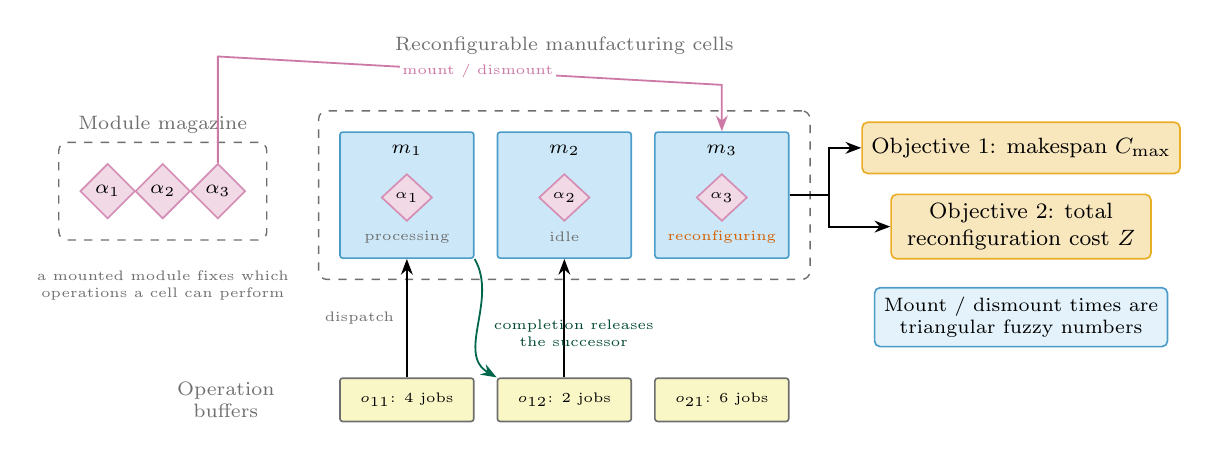
\begin{tikzpicture}

% ---------------- module magazine ----------------
\node[modnode, minimum size=7mm] (mo1) at (-5.4,1.5) {$\alpha_1$};
\node[modnode, minimum size=7mm] (mo2) at (-4.7,1.5) {$\alpha_2$};
\node[modnode, minimum size=7mm] (mo3) at (-4.0,1.5) {$\alpha_3$};
\node[note] at (-4.7,2.35) {Module magazine};
\node[tinynote, align=center] at (-4.7,0.30)
  {a mounted module fixes which\\operations a cell can perform};

% ---------------- reconfigurable cells ----------------
\node[note] at (0.4,3.35) {Reconfigurable manufacturing cells};

% The status label lives inside the cell box, so nothing can collide with
% the dashed group border.
\foreach \i/\x/\mod/\st/\c in {%
    1/-1.6/$\alpha_1$/processing/oigray,
    2/0.4/$\alpha_2$/idle/oigray,
    3/2.4/$\alpha_3$/reconfiguring/oivermilion} {
  \node[macnode, minimum width=17mm, minimum height=16mm] (M\i) at (\x,1.45) {};
  \node[font=\scriptsize] at (\x,2.02) {$m_\i$};
  \node[modnode, minimum size=6mm, font=\tiny] at (\x,1.42) {\mod};
  \node[font=\tiny, text=\c] at (\x,0.92) {\st};
}

% mount / dismount routed clear of the cell group
\draw[arrow, draw=oipurple] (mo3.north) -- ++(0,1.35) -- (2.4,2.85) -- (M3.north);
\node[tinynote, text=oipurple, whitebg] at (-0.7,3.02) {mount / dismount};

% ---------------- buffers and job flow ----------------
\foreach \i/\x/\lab in {1/-1.6/{$o_{11}$: 4 jobs}, 2/0.4/{$o_{12}$: 2 jobs},
                        3/2.4/{$o_{21}$: 6 jobs}} {
  \node[draw, rounded corners=1pt, minimum width=17mm, minimum height=5.5mm,
        fill=oiyellow!30, draw=oigray, line width=0.6pt, font=\tiny] (B\i) at (\x,-1.15) {\lab};
}
\node[note, align=center] at (-3.9,-1.15) {Operation\\buffers};

\draw[arrow] (B1.north) -- (M1.south);
\draw[arrow] (B2.north) -- (M2.south);
\node[tinynote, left=0.4mm of $(B1.north)!0.5!(M1.south)$] {dispatch};

% A completed operation releases its successor into the next buffer. Drawn as a
% short curve between the two columns so it crosses no other arrow.
\draw[arrow, draw=oigreen!65!black]
  (M1.south east) to[out=-60, in=150] (B2.north west);
\node[tinynote, text=oigreen!45!black, align=center, anchor=west] at (-0.62,-0.30)
  {completion releases\\the successor};

% ---------------- objectives ----------------
\node[keyblock, minimum width=33mm] (obj1) at (6.2,2.05)
  {Objective 1: makespan $\Cmax$};
\node[keyblock, minimum width=33mm] (obj2) at (6.2,1.05)
  {Objective 2: total\\reconfiguration cost $Z$};
\node[block, minimum width=33mm, font=\scriptsize] (unc) at (6.2,-0.10)
  {Mount / dismount times are\\triangular fuzzy numbers};

\draw[arrow] (M3.east) -- ++(5mm,0) |- (obj1.west);
\draw[arrow] (M3.east) -- ++(5mm,0) |- (obj2.west);

\begin{scope}[on background layer]
  \node[group, fit=(mo1)(mo3)] {};
  \node[group, fit=(M1)(M3)] {};
\end{scope}
\end{tikzpicture}
\end{document}
